\documentclass[12pt]{article}
\usepackage{epsf}
\usepackage{amssymb}
\usepackage{enumitem}
\usepackage{amsmath}
\usepackage{tikz}
\usetikzlibrary{automata, positioning, arrows}

\title{aashlock-331-hw3}
\author{Aren Ashlock}
\date{February 11, 2024}

\setlength{\oddsidemargin}{-0.25in}
\setlength{\topmargin}{-0.5in}
\setlength{\headheight}{0cm}
\setlength{\headsep}{0cm}
\setlength{\textheight}{10in}
\setlength{\textwidth}{7in}
\setlength{\topskip}{0cm}

\begin{document}

\noindent\textbf{ComS 331 \quad Spring 2024 \quad Name: Aren Ashlock}

\begin{enumerate}

%----------------------------------- Q1 DONE -----------------------------------

\item $L = \{a_0b_0 ... a_{n-1}b_{n-1} | n \in \mathbb{N} \wedge \forall i, 0 \leq i < n, a_i \in \{0,1\} \wedge b_i \in \{0,1\} \wedge (a_{n-1}...a_0)_2 > (b_{n-1}...b_0)_2\}$

\begin{tikzpicture}
    [node distance = 2cm]
    \node[state, initial, initial text=] (sA) {A};
    \node[state, right of=sA] (sB) {B};
    \node[state, below of=sA] (sC) {C};
    \node[state, below of=sC, accepting] (sD) {D};
    \node[state, right of=sC] (sE) {E};
    \node[state, right of=sD] (sF) {F};

    \path[->] (sA) edge [midway, above] node {$0$} (sB);
    \path[->] (sB) edge [midway, above, bend right=50] node {$0,1$} (sA);
    \path[->] (sA) edge [midway, left] node {$1$} (sC);
    \path[->] (sC) edge [midway, left, bend left=50] node {$1$} (sA);
    \path[->] (sC) edge [midway, left] node {$0$} (sD);
    \path[->] (sE) edge [midway, right] node {$1$} (sA);
    \path[->] (sD) edge [midway, left, bend left=20] node {$0$} (sE);
    \path[->] (sE) edge [midway, right] node {$0$} (sD);
    \path[->] (sD) edge [midway, above, bend left=10] node {$1$} (sF);
    \path[->] (sF) edge [midway, below, bend left=10] node {$0,1$} (sD);
\end{tikzpicture}

%-------------------------------------------------------------------------------

%----------------------------------- Q2 DONE -----------------------------------

\item "The language which the final 4 bits are less than 8 (in decimal)."\\
$L = \{a_0a_1...a_{n-2}a_{n-1} | n \in \mathbb{N} \wedge n \geq 4 \wedge \forall i, 0 \leq i < n, a_i \in \{0,1\} \wedge (a_{n-4}a_{n-3}a_{n-2}a_{n-1})_2 < 8_{10}\}$

\begin{tikzpicture}
    [node distance = 2cm]
    \node[state, initial, initial text=] (sA) {A};
    \node[state, right of=sA] (sB) {B};
    \node[state, right of=sB] (sC) {C};
    \node[state, right of=sC] (sD) {D};
    \node[state, right of=sD, accepting] (sE) {E};

    \path[->] (sA) edge [loop above] node {$0,1$} (sA);
    \path[->] (sA) edge [midway, above] node {$0$} (sB);
    \path[->] (sB) edge [midway, above] node {$0,1$} (sC);
    \path[->] (sC) edge [midway, above] node {$0,1$} (sD);
    \path[->] (sD) edge [midway, above] node {$0,1$} (sE);
\end{tikzpicture}

%-------------------------------------------------------------------------------

%----------------------------------- Q3 DONE -----------------------------------

\item Prove or disprove: if a language $L \subseteq \Sigma^*$ is recognized by a FA, then there is a NFA $M = (K, \Sigma, \delta, s_0, F)$ with $|F| = 1$ such that $L = L(M)$.

\color{blue} Let's start by defining an FA which recognizes the language $L$. This is defined as $M' = (K', \Sigma, \delta', s_0', F')$.

Then, we construct the NFA $M = (K, \Sigma, \delta, s_0, F)$ where $K = K' \cup \{k_f\}$, $s_0 = s_0'$, and $F = \{k_f\}$. This satisfies the condition that $|F| = 1$. For $\delta$, we construct it as follows: $\forall k \in K', \forall x \in \Sigma, \delta(k, x) = \delta'(k, x)$ AND $\forall k \in F', \delta(k, \epsilon) = \{k_f\}$.

As a result, we get an NFA with only 1 final state. This NFA is essentially the same in terms of states and transitions. However, we added in a new, singular final state that each of the final states from the FA transition to by $\epsilon$. This ends up accepting the same language as the FA, but with only 1 final state.

\textbf{Therefore,} there is a NFA $M = (K, \Sigma, \delta, s_0, F)$ with $|F| = 1$ such that $L = L(M)$. \color{black}

%-------------------------------------------------------------------------------

%----------------------------------- Q4 DONE -----------------------------------

\item \textbf{Equivalent} (non-minimized) DFA $M'$:

\begin{tikzpicture}
    [node distance = 3cm]
    \node[state, initial, initial text=] (s1) {\{AB\}};
    \node[state, right of=s1, accepting] (s2) {\{CD\}};
    \node[state, below of=s1, accepting] (s3) {\{ABCD\}};
    \node[state, right of=s3, accepting] (s4) {\{BCD\}};

    \path[->] (s1) edge [loop above] node {$a$} (s1);
    \path[->] (s1) edge [midway, above] node {$b$} (s2);
    \path[->] (s2) edge [midway, right, bend left=10] node {$a$} (s4);
    \path[->] (s4) edge [midway, left, bend left=10] node {$b$} (s2);
    \path[->] (s3) edge [midway, above] node {$b$} (s2);
    \path[->] (s4) edge [midway, above] node {$a$} (s3);
    \path[->] (s3) edge [loop left] node {$a$} (s3);
\end{tikzpicture}

\textbf{Minimized} DFA $M''$:

\begin{tikzpicture}
    [node distance = 4cm]
    \node[state, initial, initial text=] (s1) {\{AB\}};
    \node[state, right of=s1, accepting] (s2) {\{CD\}};
    \node[state, right of=s2, accepting] (s3) {\{ABCD, BCD\}};

    \path[->] (s1) edge [loop above] node {$a$} (s1);
    \path[->] (s1) edge [midway, above] node {$b$} (s2);
    \path[->] (s2) edge [midway, above, bend left=10] node {$a$} (s3);
    \path[->] (s3) edge [midway, below, bend left=10] node {$b$} (s2);
    \path[->] (s3) edge [loop right] node {$a$} (s3);
\end{tikzpicture}

\textbf{English}: "The language which all strings contain at least 1 $b$ and there are no consecutive $b$ inputs."

%-------------------------------------------------------------------------------

\end{enumerate}
\end{document}